\documentclass[final]{beamer}
  \mode<presentation>
  {
% you can chose your theme here:
%  \usetheme{Aachen}
  \usetheme{I6dv}
%  \usetheme{I6pd}
%      \usetheme{Berlin}
%  \usetheme{I6pd2}
%  \usetheme{I6td}
%  \usetheme{Oldi6}
}
%\graphicspath{{figures/}}

\usepackage{setspace} 
\usepackage{wrapfig}
\usepackage[numbers, compress]{natbib}

\usepackage{graphicx}

\usepackage{subcaption}
\usepackage{lipsum}
\usepackage{times}
\usepackage{booktabs}       % professional-quality tables

\usepackage{makecell}
\usepackage{blindtext}
\usepackage{amsmath,amssymb}
\usepackage{booktabs, array}
\usepackage{algorithm}
\usepackage{algorithmic}
\usepackage{dsfont}
\usepackage{wasysym}
\usepackage{fancybox}
\usepackage[english]{babel}
\usepackage[latin1]{inputenc}
\usepackage{mathtools}
\usepackage[orientation=portrait,size=a0,scale=1]
{beamerposter}  % e.g. custom size poster
  \title{{Toward Bayesian permutation inference for identifying neurons in \textit{C. elegans}.}}
  \author[]{Gonzalo E. Mena$^{1,*}$, Scott Linderman $^{1,*}$, David Belanger $^2$, Jasper Snoek $^2$, John Cunningham$^{1,3}$, Liam Paninski$^{1,3}$}
  \institute[]{\linebreak 1. Department of Statistics, Columbia University, New York, NY, USA 2. Google Brain, Cambridge, MA.
   3. Center for Theoretical Neuroscience and Grossman Center for the Statistics of Mind, Columbia University, New York, NY, USA.}

\newcommand{\logit}{\text{logit}}
\newcommand{\Bernoulli}{\text{Bernoulli}}
\newcommand{\N}{\mathcal{N}}
\newcommand{\p}{\text{p}}
\newcommand{\bfx}{\mathbf{x}}
\newcommand{\bfy}{\mathbf{y}}
\newcommand{\bfm}{\mathbf{m}}
\newcommand{\bfb}{\mathbf{b}}
\newcommand{\bfh}{\mathbf{h}}
\newcommand{\bfd}{\mathbf{d}}




\makeatletter
    \newenvironment{withoutheadline}{
        \setbeamertemplate{headline}[default]
        \def\beamer@entrycode{\vspace*{-\headheight}}
    }{}
\makeatother


\begin{document}

 \begin{frame}[allowframebreaks]

     \begin{minipage}[htp][1\textheight][t]{\textwidth}

        \begin{columns}[t]
             \hspace{1cm} 
            \begin{column}{.5\linewidth}
              \begin{block}{Summary}
                        
	               \textbf{Overarching goal}
              		\begin{itemize}
		\item State and infer Bayesian hierarchical models for the activity in C.elegans	combining information (calcium traces) from several worms.   
		\item This is possible as C.elegans nervous system is stereotypical, neurons and connectome don't change across individuals.
		 \end{itemize}
		 	 \textbf{Challenge}
              		\begin{itemize}
		\item If neural identity is known for each trace, one can apply standard bayesian methodology
		\item In practice, laborious human supervision is needed to match recorded traces to canonical neural identities (i.e. names) \end{itemize}

		\textbf{Our contribution}
	\begin{itemize}
	\item We Developed three methods for learning latent matchings. These can be used in variational inference (VI) to jointly estimate a dynamical system and the matching between traces and true neural identities.
	\item Potentially it may serve to automatize the matching procedure.
	\item From a statistical machine learning perspective, the relevance is that outperforms a simple MCMC sampler for permutations.
	\end{itemize}
	\textbf{Future work}
	\begin{itemize}
	\item We used real connectome a position information. In the future we plan to use real traces.
	\item Two new levels of complexity: partially observed brain recordings, more sophisticated dynamical systems.
	\end{itemize}
	   
	 
	    \end{block}
	    
\begin{block}{Model}
We focus on a simple linear autoregressive
model for neural dynamics,
\begin{align}
  \widetilde{Y}_t^{(j)} &= (W \odot A) \widetilde{Y}_{t-1}^{(j)} + \epsilon_t^{(j)},
\end{align}
where~$W \in \mathbb{R}^{N \times N}$ is the weight matrix we wish to infer;
$A \in \{0,1\}^{N \times N}$ is the known adjacency matrix or connectome;
$\odot$ denotes element-wise multiplication;
$\epsilon_t^{(j)} \sim \mathcal{N}(0, \sigma^2 I)$;
and~$\widetilde{Y}_t^{(j)} \in \mathbb{R}^N$ is the measured neural activity
at time~$t$ in worm~$j$.  The catch is that~$\widetilde{Y}_t^{(j)}$ is
assumed to be in canonical order; i.e. in the same order as the rows and
columns of~$W$ and~$A$. We actually observe,
\begin{align}
  Y_t^{(j)} &= P^{(j)} \widetilde{Y}_t^{(j)},
\end{align}
vectors that are permuted by matrix~$P^{(j)}$. In order to learn about~$W$,
we must also infer the permutation matrices. We place a Gaussian prior on~$W$.

\vspace{0.5cm}
The permutation matrices are constrained by side
information: we use neural position along the worm's
body to constrain the possible neural identities for a given recorded
neuron. We only allow an observed neuron to be mapped to a known
identity if the observed location is within~$\eta$ of the expected
location.  

\vspace{0.5cm}
This is illustrated in Fig.~\ref{fig:1}B. We represent
these constraints with the matrix~$\mathcal{C}^{(j)}$ so that
$\mathcal{C}^{(j)}_{mn}=1$ if and only if observed neuron $m$ is
within~$\eta$ of canonical neuron $n$'s expected location.  An
example is shown in Figure \ref{fig:1}C. We let~$P^{(j)}$ have a
uniform prior over the set of matrices allowable under the given
constraints.

We aim to perform posterior inference of $p(\{W,P^{(j)}\} \, | \, A, \{Y^{(j)}\})$.
\end{block}

	 	             	    
\begin{block}{Experimental setup}

\begin{figure}[t]
  \centering
  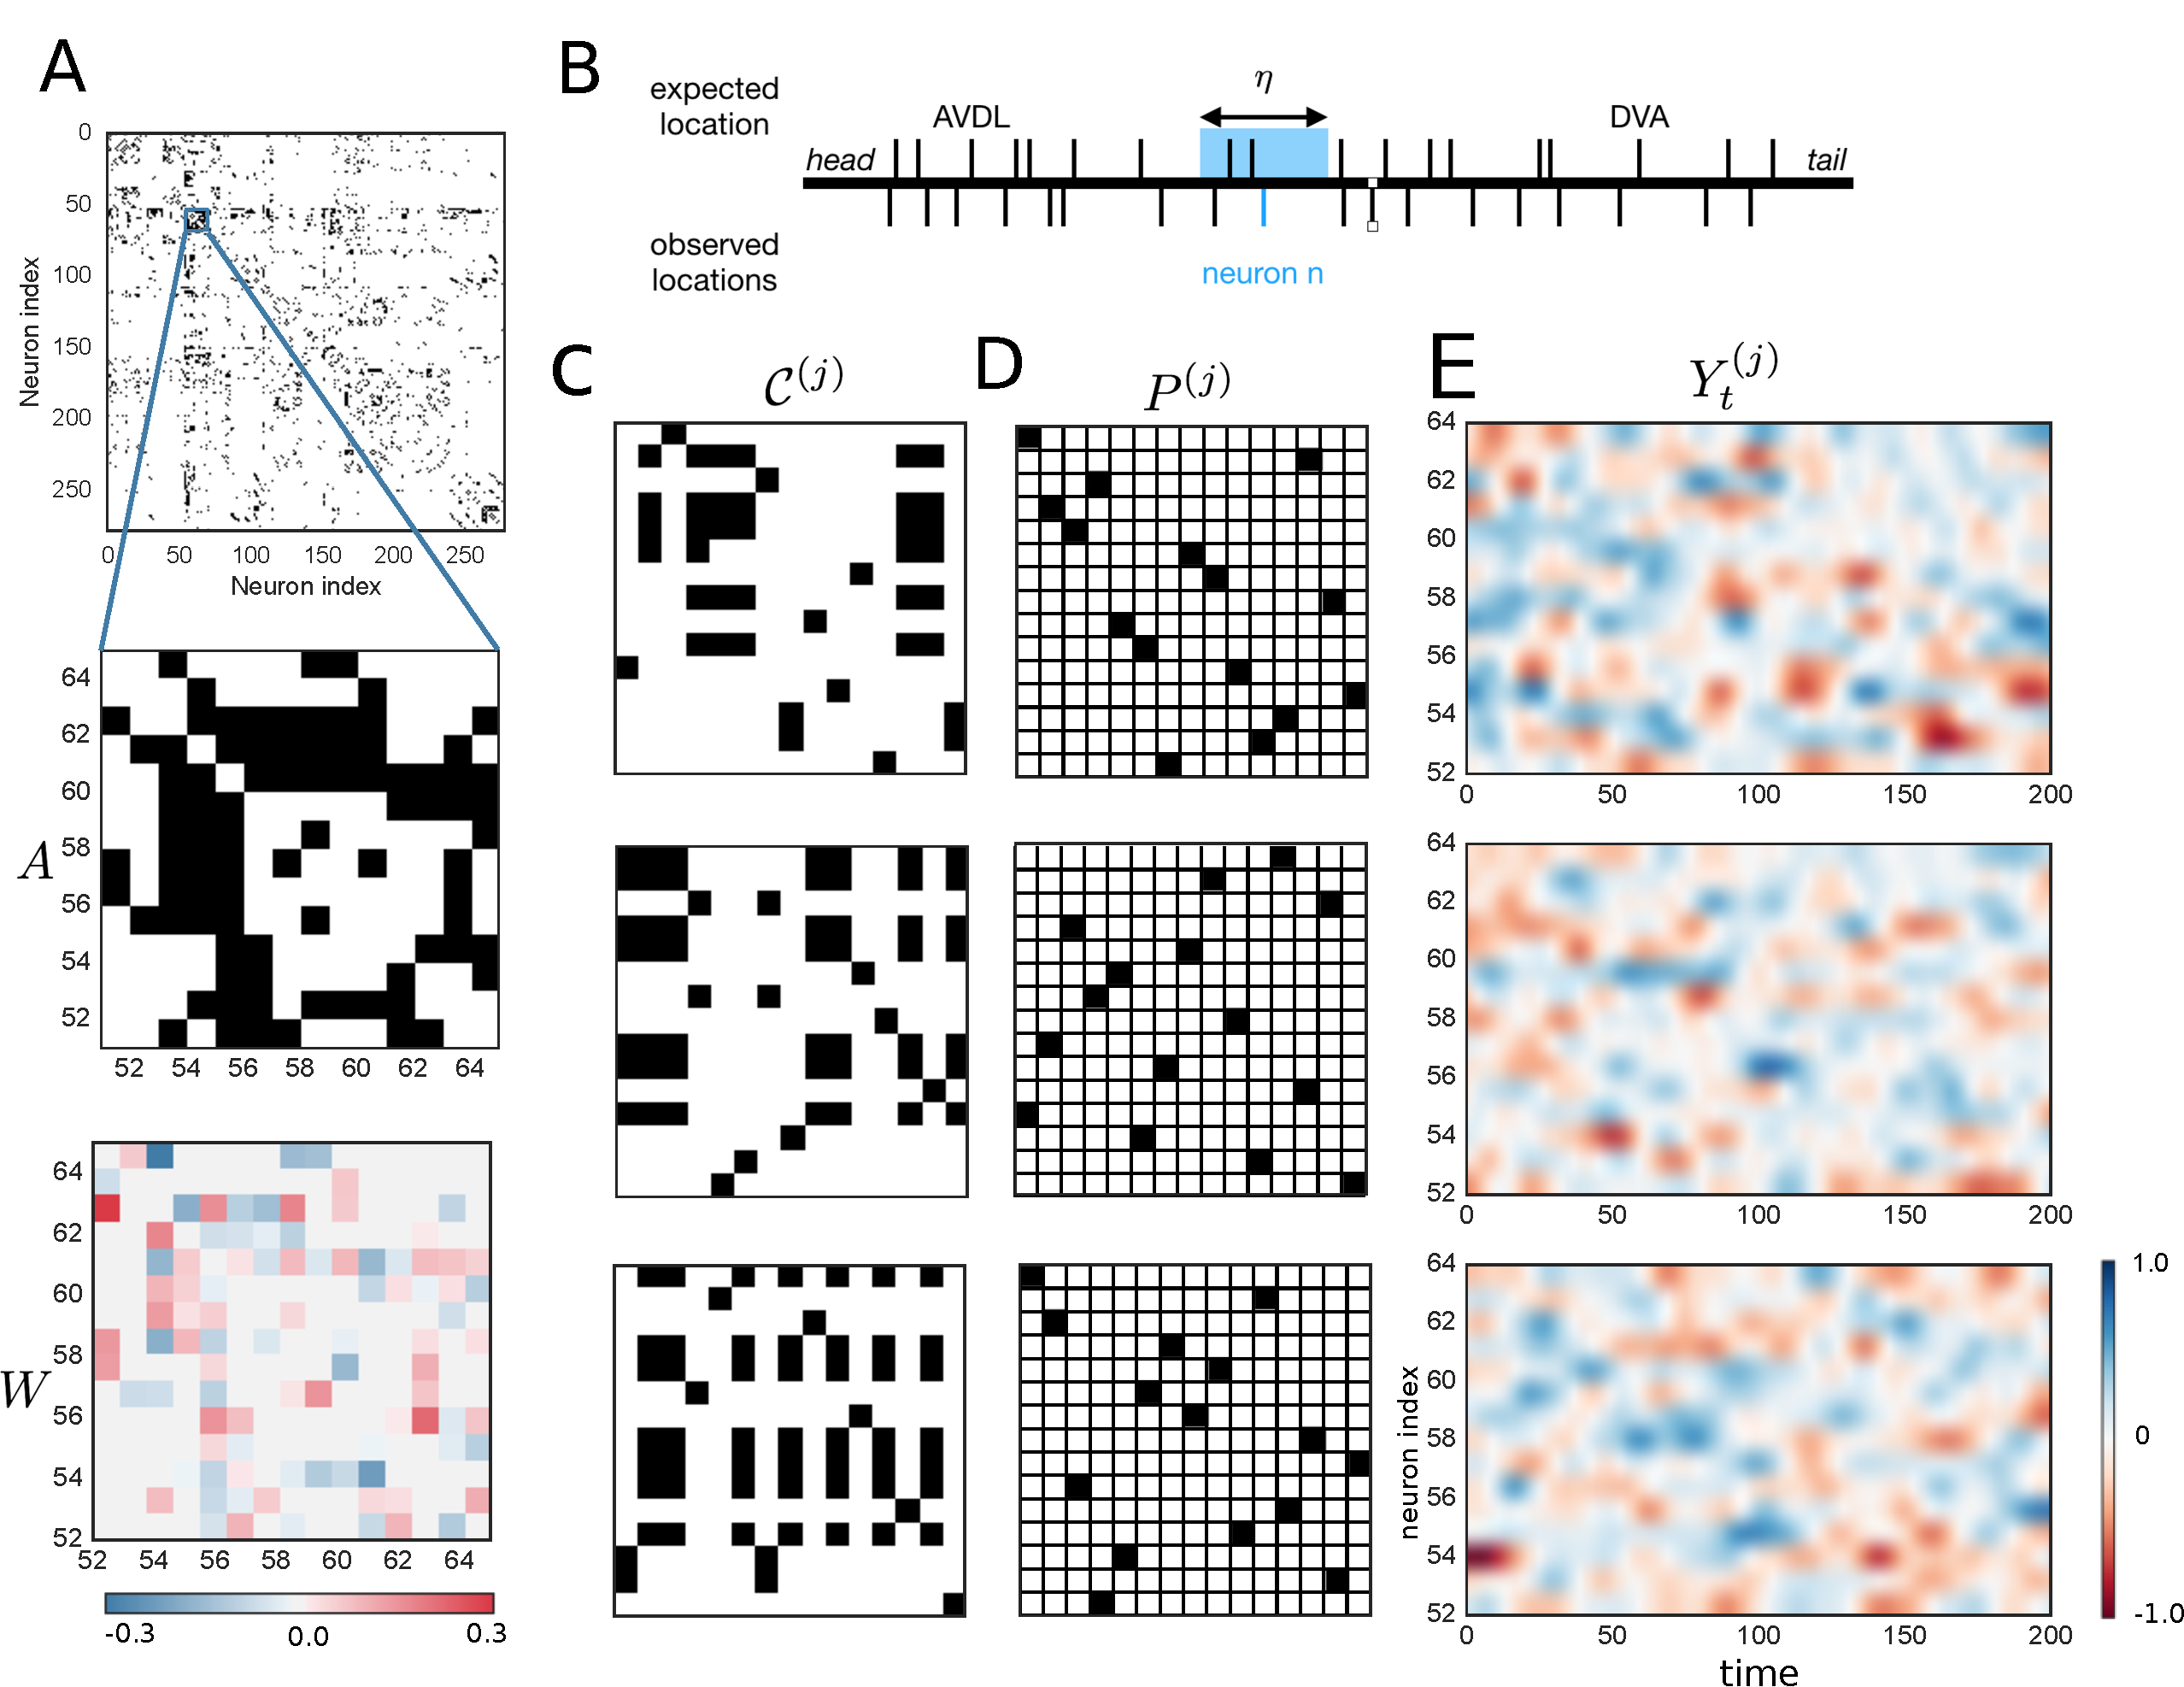
\includegraphics[width=0.7\textwidth]{figs/Figure3.pdf} 
  \caption{\small \textit{Hierarchical Bayesian framework}.  \textbf{A} We
    are given the actual adjacency matrix $A$ from
    \cite{varshney2011structural}. The full matrix is shown (top)
    along with a zoom-in to 14 neurons (center).  We wish to infer the
    corresponding weight matrix~$W$, an example of which is shown
    below.  \textbf{B} We also know the typical locations of the
    neurons \cite{white1986structure,wormatlas}. 
    Given observed
    locations, we constrain possible assignments to neuron identities
    within~$\eta$ of the observed location.  \textbf{C} These
    constraints are represented as a matrix $\mathcal{C}^{(j)}$ for
    worm~$j$ which specifies possible assignments of observed neurons
    to known identities. This illustration shows three worms.
    \textbf{D} To infer the weights, we must first infer the
    permutation $P^{(j)}$ that matches the observed neurons in
    worm~$j$ to the set of known identities.  \textbf{E} The observed
    data is a matrix~$Y^{(j)}$ whose rows are ordered according to the
    order in which neurons were observed in that worm.  The
    permutation matrix maps this to the canonical ordering of the
    adjacency and weight matrices. Given~$\{Y^{(j)}\}_{j=1}^J$
    and~$A$, we infer~$\{P^{(j)}\}_{j=1}^J$ and~$W$.}

\label{fig:1}
\end{figure}



	   \end{block}
   	
	  \begin{block}{Three reparameterizations for permutations}
We developed three reparameterizations for permutations; all of them Inspired by the recently introduced methods by \cite{Jang2016,Maddison2016}. Briefly, one can relax the \emph{hard} sample of a category using the \emph{soft}max, leading to a probability-simplex valued distribution, the so-called \emph{Concrete} or \emph{Gumbel-Softmax} distributions. These are proposed as alternative to REINFORCE \cite{Williams1992} for learning latent discrete variables in stochastic computation graphs, e.g. approximate posterior inference. Specifically, one applies the the \emph{reparameterization trick} machinery developed in \cite{Kingma2014}.

\vspace{0.5cm}
Critically, REINFORCE cannot be used here, as it requires the evaluation of an intractable partition function for any non-trivial distribution on permutations. Extending \emph{Gumbel-Softmax} is then the only choice. Two of our extensions, \emph{Stick-breaking} and \emph{rounding}, have tractable densities \cite{Linderman2017}. The third one, \emph{Gumbel-Sinkhorn} does not does not. However, in practice the latter leads to best results as it allows a more efficient use of a regularizing prior \cite{Mena2017}. 

In all relaxations we are particularly concerned with $\mathcal{B}_N$, the Birkhoff polytope or set of doubly-stochastic matrices. $\mathcal{B}_N$ is the convex hull of the set of permutation matrices; it is therefore the most suited to conceive relaxations.
	  \end{block}
            \end{column}    


            
            \begin{column}{.5\linewidth}
           
	              
	  
	    \begin{block}{Stick-Breaking and Rounding}
	    On the stick-breaking
method, we generalize the standard construction on the simplex \cite{linderman2015dependent} to
stick-breaking of $\mathcal{B}_N$. We show how to consistently
``break the stick'' while satisfying both the row and column
constraints that characterize a doubly stochastic matrix. For the
rounding construction, we start with a noise distribution and force it
to be close to permutation matrices by rounding them towards the
extreme-points of the Birkhoff polytope (i.e. permutation
matrices). 

           	 \begin{figure}
	    	\centering
		{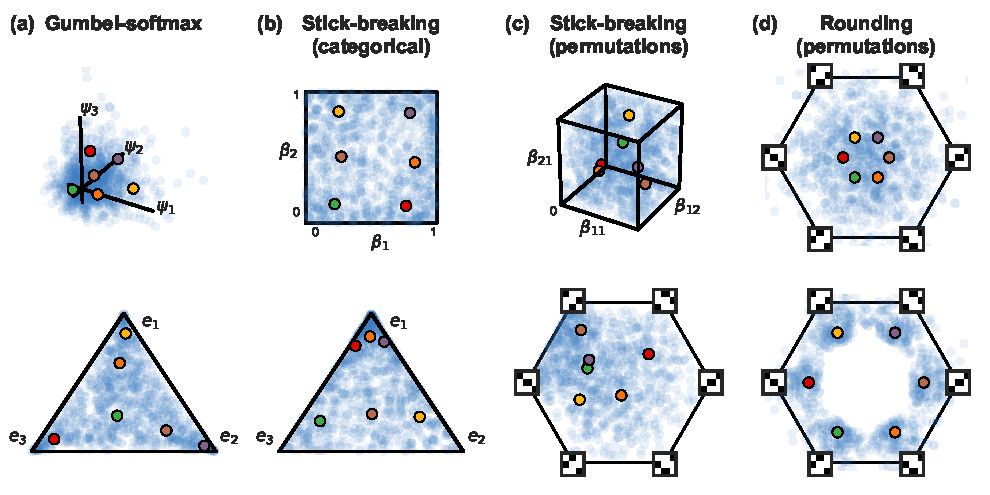
\includegraphics[width=0.8\textwidth]{figs/Figure1.pdf}}
		 \caption{(a)~The Gumbel-softmax, or ``Concrete'' transformation maps
    Gumbel r.v.'s (blue dots) to points in the
    simplex by applying the softmax.  Colored
    dots are random variates that aid in visualizing the
    transformation.  (b)~Stick-breaking offers and alternative
    transformation for categorical inference, but the ordering of
    the stick-breaking induces an asymmetry in the transformation.
    (c)~We extend this stick-breaking transformation to reparameterize
    the Birkhoff polytope, i.e. the set of doubly-stochastic
    matrices. We show how~$\mathcal{B}_3$ is reparameterized in terms of
    matrices~$B \in [0,1]^{2 \times 2}$ These points are mapped to
    doubly-stochastic matrices, which we have projected
    onto~$\mathbb{R}^2$ below.  (d)~Finally, we derive a ``rounding'' transformation
    that moves points in~$\mathbb{R}^{N \times N}$ nearer to the closest
    permutation matrix. This is more symmetric, but does not map strictly onto ~$\mathcal{B}_N$.
  }
\label{fig:transforms}
	\end{figure}


	  
\end{block}
	
	     
	\begin{block}{Gumbel-Sinkhorn ($\mathcal{G.S}$) distribution}
Finally, for the Gumbel-Sinkhorn method we notice that the
so-called \emph{Sinkhorn operator} $S(\cdot)$, or infinite and successive row and
column normalization of a matrix approximates the choice of a permutation through the matching operator $M(X)$; i.e. $M(X)=\lim_{\tau\rightarrow 0} S(X/\tau)$. By adding Gumbel noise we conceive the Gumbel Matching distribution and its approximation, the  \emph{G.S.} distribution.
distribution, which approximates the sampling of a discrete
distribution over permutations. 
			\begin{figure}
         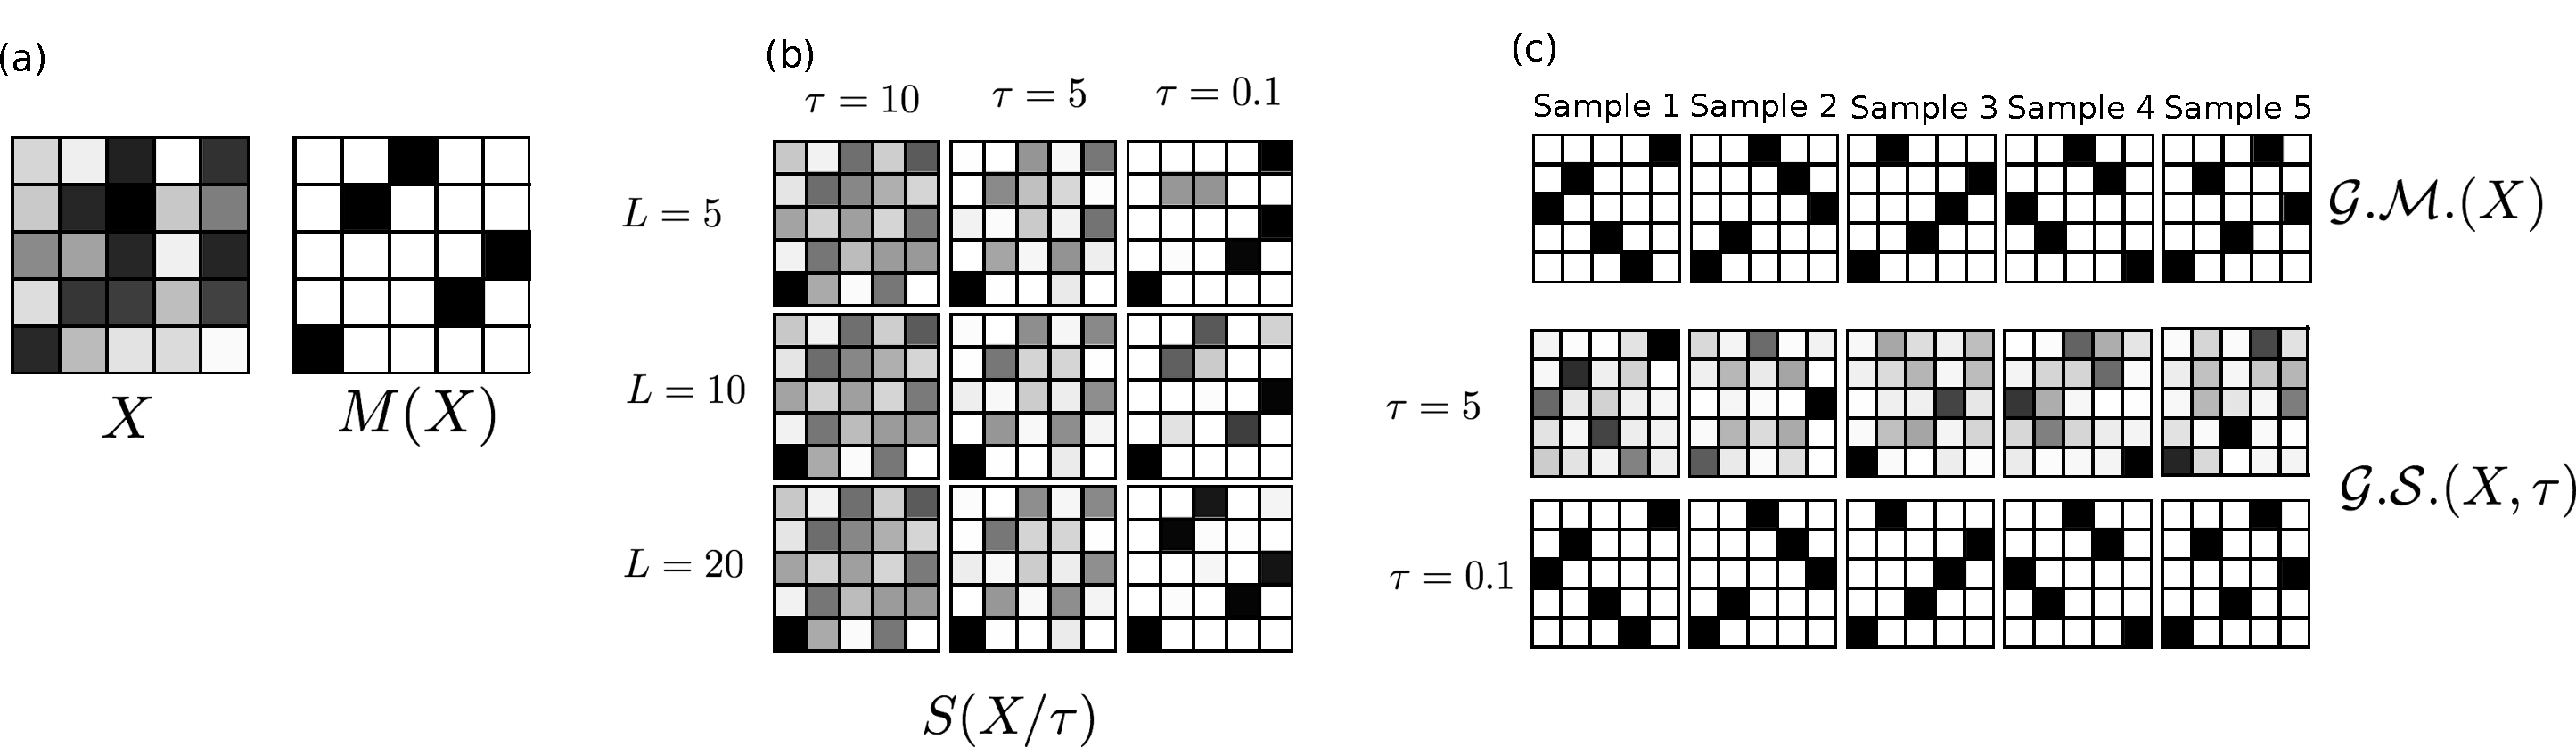
\includegraphics[trim = 0cm 0cm 0mm 0.0cm, clip=true, width=0.8\textwidth]{figs/Figure2.pdf}
	 \caption{Illustrating the Matching and Sinkhorn operators, and the Gumbel-Matching and Gumbel-Sinkhorn distributions. Each 5x5 grid represents a matrix, with the shading indicating cell values (a) Matching operator $M(X)$ applied to a parameter matrix $X$. (b) Sinkhorn Operator $S(X/\tau)$ approximating $M(X)$ for different temperature $\tau$ and number of Sinkhorn iterations, $L$. (c). First row: samples from the Matching Sinkhorn distribution. Second and third rows: samples from the Gumbel-Sinkhorn distribution at two temperatures. At low temperature, both distributions are indistinguishable.}
 \label{fig:figure2}
 \end{figure} 
            \end{block}	
             

      	\begin{block}{Results}
	
We compared against three alternatives: (i) na\"ive variational inference,
where we do not enforce the constraint that $P^{(j)}$ be a permutation
and instead treat each row of~$P^{(j)}$ as a Dirichlet distributed
vector; (ii) MCMC, where we alternate between sampling from the
conditionals of $W$ (Gaussian) and ${P^{(j)}}$, from which one can
sample by proposing local swaps, as described in \cite{Diaconis2009},
and (iii) maximum a posteriori estimation (MAP). 

We found that our method outperforms these alternative
approaches. When there are many possible candidates (Table 1) and when
only a small proportion of neurons are known with certitude (Table 2),
variational inference via continuous relaxation with the
Gumbel-Sinkhorn method performs best.  
\begin{table}[t]
     \caption{Accuracy in the C.elegans neural identification problem, for varying mean number of candidate neurons (10, 30, 45, 60) and number of worms.}
   \label{table:celeganssup}

   \centering
  \begin{tabular}{lllllllllll}
    & \multicolumn{2}{c}{10} & \multicolumn{2}{c}{30} &   \multicolumn{2}{c}{45} & \multicolumn{2}{c}{60} \\
    \cmidrule(lr){2-3} \cmidrule(lr){4-5} \cmidrule(lr){6-7} \cmidrule(lr){8-9}
& 1 worm & 4 worms & 1 Worm & 4 worms & 1 worm & 4 worms & 1 worms & 4 worms \\
    \midrule 
    NAIVE VI &.34 & .32 & .16 & .16 & .13 & .12 & .11 & .12 \\
   MAP   & .34 & .32  &.17 &.17& .14 & .13 & .13 & .12 \\
    MCMC   & .34 & .65  &.18 &.28& .14 & .17 & .13 & .15 \\
  
    VI   & \textbf{.79} & \textbf{.94} & \textbf{.4} & \textbf{.69} & \textbf{.25}&  \textbf{.51} & \textbf{.21} & \textbf{.44}\\
 
    \bottomrule
  \end{tabular}
\end{table}


\begin{table}[t]
  \caption{Accuracy in inferring true neural identity for different of
    proportion of known neurons and $\eta$.
  }
   \label{table:celegans}
   \centering
   \begin{tabular}{lllllllll}
    & \multicolumn{2}{c}{40.\%} & \multicolumn{2}{c}{30.\%} & \multicolumn{2}{c}{20.\%} & \multicolumn{2}{c}{10.\%}\\
    \cmidrule(lr){2-3} \cmidrule(lr){4-5} \cmidrule(lr){6-7} \cmidrule(lr){8-9}
    & $\eta=0.1$ & $\eta=0.2$ & $\eta=0.1$ & $\eta=0.2$  & $\eta=0.1$ & $\eta=0.2$  & $\eta=0.1$ & $\eta=0.2$ \\
    \midrule 
    Naive VI & .43 & .41 & .33 & .31 & .23 & .22 & .12 & .1 \\
    MAP & .42 & .41  &.33 &.32& .23 & .22 & .12 & .11 \\
    MCMC   & .85 & .80  &.52 &.46& .3 & .26 & .15 & .12 \\
   %   \shortstack{Gumbel-Sinkhorn, no regularization (VI)} & .96 & .93 & .88 & .78 &  .69 & .52 & .39 & .21 \\
   %Rounding (VI)& \textbf{.97} & \textbf{.95} & \textbf{.90} & .84 & .75&  .\textbf{58} & \textbf{.37} & \textbf{.17} \\
    VI   & \textbf{.97} & \textbf{.96} & \textbf{.92} & \textbf{.84} & \textbf{.74} & \textbf{.58} & \textbf{.44} & \textbf{.23} \\
              \bottomrule
   \end{tabular}
\end{table}
\end{block}

\begin{block}{Conclusion}
Our results provide promising evidence that a Bayesian hierarchical
approach to the study of neural dynamics on C. elegans is feasible. We
note we made many simplifying assumptions that are not justified in
practice: first, we assumed a linear dynamical system, while actual
dynamics are highly nonlinear~\citep{Kato2015}. Fortunately, there
exist many methods for inference in nonlinear
systems~\citep{Krishnan2015, linderman2017bayesian}. Also, we assumed
all neurons were observed, while in reality we only see about 100
neurons at a time. The methods of~\citet{Soudry2015} may help
infer the weights, but reasoning about partial permutations requires
more care. 
	\end{block}


   
	     \begin{block}{References}
	     \tiny
		\bibliography{refs}
\bibliographystyle{abbrvnat}


	\end{block}
	     	   		     

	     \end{column}
	     
            
            
            
	\end{columns}
      \end{minipage}
      
       
       

      
\end{frame}

\end{document}

%%%%%%%%%%%%%%%%%%%%%%%%%%%%%%%%%%%%%%%%%%%%%%%%%%%%%%%%%%%%%%%%%%%%%%%%%%%%%%%%%%%%%%%%%%%%%%%%%%%%
%%% Local Variables: 
%%% mode: latex
%%% TeX-PDF-mode: t